%%%%%%%%%%%%%%%%%%%%%%%%%%%%%%%%%%%%%%%%%%%%%%%%%%%%%%%%%%%%%%%%%%%%%%%%%%%%%%%
%%%%%%%%%%%%%%%%%%%%%%%%%%%%%%%%%%%%%%%%%%%%%%%%%%%%%%%%%%%%%%%%%%%%%%%%%%%%%%%
\chapter{Разработка алгоритма технологии объединения абстрактной интерпретации 
и метода ограниченной проверки моделей}
\label{chapter:algorithm}
%%%%%%%%%%%%%%%%%%%%%%%%%%%%%%%%%%%%%%%%%%%%%%%%%%%%%%%%%%%%%%%%%%%%%%%%%%%%%%%
%%%%%%%%%%%%%%%%%%%%%%%%%%%%%%%%%%%%%%%%%%%%%%%%%%%%%%%%%%%%%%%%%%%%%%%%%%%%%%%
В соответствии с поставленными задачами необходимо разработать технологию
объединения АИ и BMC. Технология состоих из нескольких этапов:
\begin{itemize}
\item интерпретация исходного кода программы;
\item проверка программы на наличие ошибок по результатам АИ;
\item интерпретация упрощенного представления программы;
\item проверка упрощенного представления программы на наличие ошибок по 
результатам АИ;
\end{itemize}

В данном разделе рассматриваются модели представления кода, для которых 
выполнялась разработка алгоритмов и описываются основные идеи, положенные в их
основу.

%%%%%%%%%%%%%%%%%%%%%%%%%%%%%%%%%%%%%%%%%%%%%%%%%%%%%%%%%%%%%%%%%%%%%%%%%%%%%%%
\section{Модель представления кода исходной программы}
%%%%%%%%%%%%%%%%%%%%%%%%%%%%%%%%%%%%%%%%%%%%%%%%%%%%%%%%%%%%%%%%%%%%%%%%%%%%%%%

%%%%%%%%%%%%%%%%%%%%%%%%%%%%%%%%%%%%%%%%%%%%%%%%%%%%%%%%%%%%%%%%%%%%%%%%%%%%%%%
\subsection{Система LLVM}
%%%%%%%%%%%%%%%%%%%%%%%%%%%%%%%%%%%%%%%%%%%%%%%%%%%%%%%%%%%%%%%%%%%%%%%%%%%%%%%
LLVM (Low Level Virtual Machine) --- универсальная система анализа, 
трансформации и оптимизации программ, реализующая виртуальную машину с RISC-
подобными инструкциями. Центральным звеном LLVM является так называемое 
промежуточное представление (Intermediate Representation, IR), представляющее 
собой строго типизированный мета-ассемблер с бесконечным числом доступных для 
использования регистров.  Такая форма представления кода в LLVM (в виде IR) 
позволяет производить большое количество оптимизаций прямо над промежуточным 
представлением без необходимости учета особенностей исходного языка 
программирования, а строгая система типов делает код удобным для восприятия и 
позволяет производить преобразования, которые не представляется возможным 
выполнить при обычном трехадресном нетипизированном представлении кода.

Одной из самых важных частей LLVM является система проходов~\cite{llvmpass}. 
Проходы отвечают за трансформацию и оптимизацию промежуточного представления и 
объединяют результаты различных анализов для их использования в дальнейших 
преобразованиях.

Программы в LLVM представляются в виде набора отдельных модулей. Каждый модуль 
состоит из функций, глобальных переменных и дополнительных метаданных. Каждая 
функция, в свою очередь, состоит из базовых блоков. Каждый базовый блок имеет 
свою метку и состоит из последовательности инструкций, заканчивающейся 
инструкцией-терминатором, которая явно передает управление в другой блок или 
завершает выполнение текущей функции. Пример представления программы в системе 
LLVM приведен на рисунке \ref{image:llvmIR}.
\begin{figure}[h!]
\center{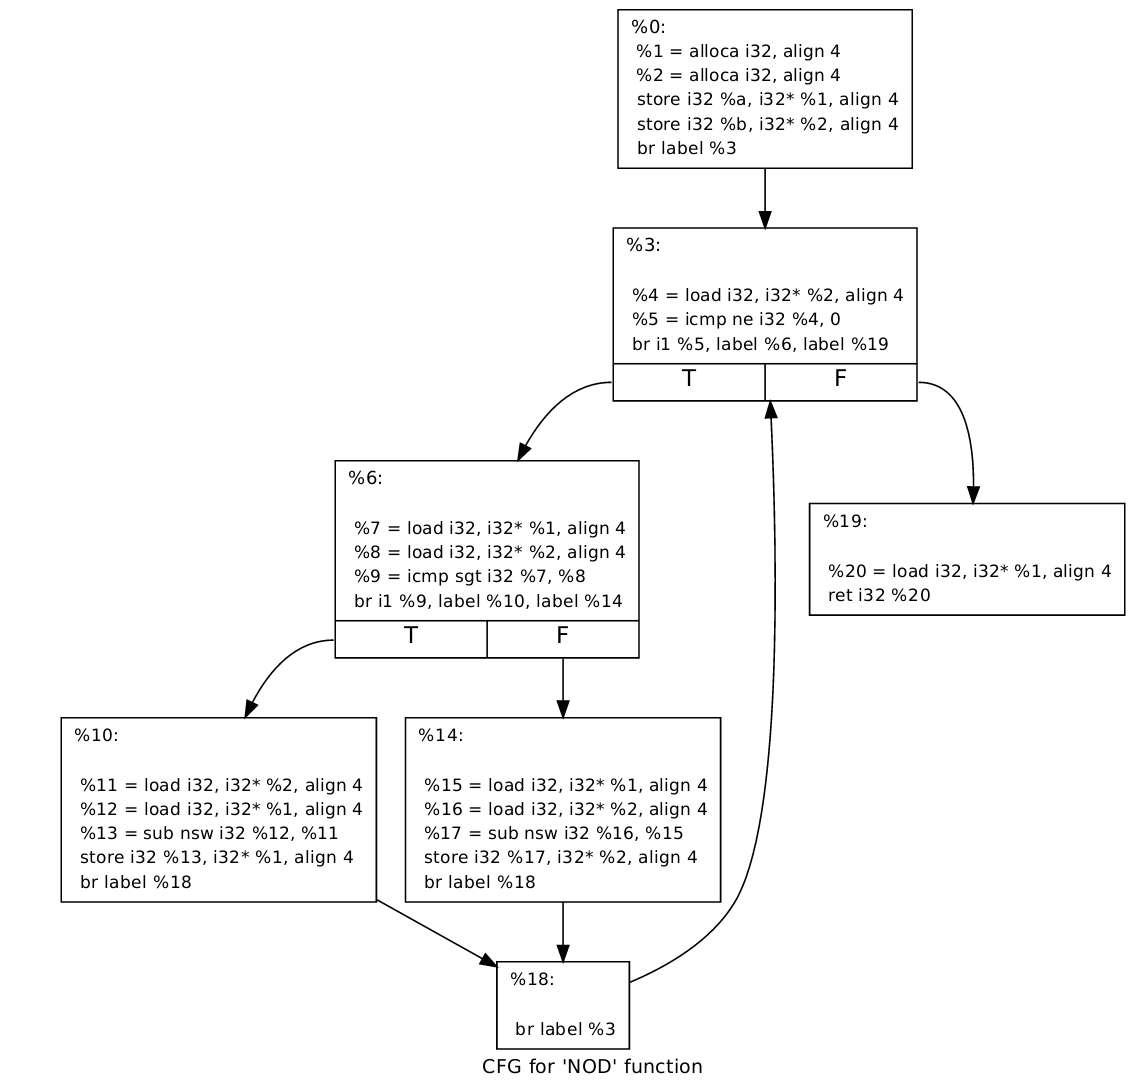
\includegraphics[width=\linewidth]{llvmIR}}
\caption{Пример представления функции в LLVM}
\label{image:llvmIR}
\end{figure}
    
Переменные исходной программы в LLVM представляются в виде регистров (память
на стеке) или в виде указателей на память (память на куче). Для регистров 
LLVM реализует статическое однократное присваивание (Static Single Assigment, 
SSA) --- форма представления кода, при которой любое значение присваивается 
только один раз. Любому регистру в LLVM можно присвоить значение только один 
раз --- при его объявлении. Для объединения потенциально различных значений 
одной и той же переменной исходной программы в SSA (то есть, и в LLVM) 
используются так называемые phi-функции, которые возвращают одно из значений в 
зависимости от того, какой блок передал управление текущему при выполнении 
программы.

Переменные в LLVM могут иметь следующие типы данных:
\begin{itemize}
\item простые типы:
    \begin{itemize}
    \item целые числа произвольной разрядности $i$. Эти числа представляются в 
    дополнительном коде, при этом различий между знаковыми и беззнаковыми 
    числами на уровне типов не делается: при необходимости с ними работают 
    разные инструкции;
    \item числа с плавающей точкой: half~(16-разрядные), float, double, quad~(
    128-разрядные) и некоторые платформозависимые типы~(например, x86\_f80);
    \item void --- пустое значение;
    \end{itemize}

\item производные типы:
    \begin{itemize}
    \item указатели;
    \item массивы;
    \item структуры~(обращение к полям структуры происходит не по имени, а по 
    номеру поля начиная с 0 в порядке их объявления);
    \item вектор --- специальный тип для упрощения SIMD-операций. Представляет 
    собой $2^n$ значений примитивного типа~(целого или с плавающей точкой);
    \item функции.
    \end{itemize}
\end{itemize}

%%%%%%%%%%%%%%%%%%%%%%%%%%%%%%%%%%%%%%%%%%%%%%%%%%%%%%%%%%%%%%%%%%%%%%%%%%%%%%%
\subsection{Представление программ в системе Borealis}
%%%%%%%%%%%%%%%%%%%%%%%%%%%%%%%%%%%%%%%%%%%%%%%%%%%%%%%%%%%%%%%%%%%%%%%%%%%%%%%
Система Borealis использует LLVM IR для компиляции, трансформации и анализа 
программ. Для упрощения взаимодействия различных компонентов Borealis 
добавляет еще один уровень промежуточного представления в виде Predicate State 
API~(PS API). Упрощенное описание PS приведено на рисунке~\ref{image:
predicateStateDefinition}.

Инструкции LLVM преобразуются в предикаты (predicate), которые выполняют 
различные операции над термами (term). Термы используются для представления 
констант, переменных, бинарных операций. Каждый терм также может являться 
операндом другого терма или предиката. Каждый терм имеет тип, который 
сооттветствует типу переменной LLVM, которую он представляет. Предикаты 
соответствуют инструкциям LLVM.
    
Предикаты в системе имеют различные типы. Всего определено 6 типов предикатов:
\begin{itemize}
\item State --- обычные предикаты, соответствующие инструкциям LLVM;
\item Path --- предикаты пути соответствуют условиям перехода в различные 
ветки программы;
\item Requires --- предикаты, использующиеся для выражения предусловий функций;
\item Ensures --- предикаты, использующиеся для выражения постусловий функций;
\item Assert --- предикаты, проверяющиеся на истинность при анализе;
\item Assume --- предикаты, позволяющие задавать утверждения, которые всегда верны.
\end{itemize}

\begin{figure}
    \begin{grammar}
    \scriptsize
    <PredicateState> ::= PredicateStateChain head:<PredicateState> 
    tail:<PredicateState>
    \alt PredicateStateChoice choices:<ListOfPredicateStates>
    \alt BasicPredicateState data:<ListOfPredicates>

    <ListOfPredicateStates> ::= <PredicateState> <ListOfPredicateStates> | 
    <empty>

    <Predicate> ::= AllocaPredicate lhv:<Term> numElems:<Term> 
    origNumElems:<Term>
    \alt DefaultSwitchCasePredicate cond:<Term> cases:<ListOfTerms>
    \alt EqualityPredicate lhv:<Term> rhv:<Term>
    \alt GlobalsPredicate globals:<ListOfTerms>
    \alt InequalityPredicate lhv:<Term> rhv:<Term>
    \alt MallocPredicate lhv:<Term> numElems:<Term> origNumElems:<Term>
    \alt SeqDataPredicate base:<Term> data:<ListOfTerms>
    \alt SeqDataZeroPredicate base:<Term> size:UInt32
    \alt StorePredicate ptr:<Term> value:<Term>
    \alt WriteBoundPredicate ptr:<Term> boundValue:<Term>
    \alt WritePropertyPredicate propName:<Term> ptr:<Term> propValue:<Term>
    
    <Term> ::= ArgumentTerm idx:UInt32 kind:<ArgumentKind>
    \alt ArgumentCountTerm
    \alt AxiomTerm term:<Term> axiom:<Term>
    \alt BinaryTerm op:<BinaryOp> lhv:<Term> rhv:<Term>
    \alt BoundTerm term:<Term>
    \alt CastTerm term:<Term> signExtend:Bool
    \alt CmpTerm op:<CmpOp> lhv:<Term> rhv:<Term>
    \alt ConstTerm | FreeVarTerm
    \alt GepTerm base:<Term> shifts:<ListOfTerms> triviallyInbounds:Bool
    \alt LoadTerm ptr:<Term>
    \alt OpaqueBigIntConstantTerm value:String
    \alt OpaqueBoolConstantTerm value:Bool
    \alt OpaqueBuiltinTerm vname:String
    \alt OpaqueCallTerm func:<Term> args:<ListOfTerms>
    \alt OpaqueFloatingConstantTerm value:Double
    \alt OpaqueIndexingTerm value:<Term> index:<Term>
    \alt OpaqueIntConstantTerm value:SInt64 | OpaqueInvalidPtrTerm
    \alt OpaqueMemberAccessTerm value:<Term> property:String indirect:Bool
    \alt OpaqueNamedConstantTerm vname:String
    \alt OpaqueNullPtrTerm | OpaqueUndefTerm 
    \alt OpaqueStringConstantTerm value:String
    \alt OpaqueVarTerm vname:String
    \alt ReadPropertyTerm propName:<Term> ptr:<Term>
    \alt ReturnPtrTerm funcName:String
    \alt ReturnValueTerm funcName:String
    \alt SignTerm value:<Term>
    \alt TernaryTerm cond:<Term> tru:<Term> fls:<Term>
    \alt UnaryTerm op:<UnaryOp> value:<Term>
    \alt ValueTerm global:Bool
    \alt VarArgumentTerm index:UInt32

    <ListOfTerms> ::= <Term> <ListOfTerms> | <empty>

    <ArgumentKind> ::= ANY | STRING
    \end{grammar}
    
\caption{Определение предикатного состояния}
\label{image:predicateStateDefinition}
\end{figure}

Predicate state ставится в соответствие каждой функции программы. При этом, 
как показано на рисунке~\ref{image:predicateStateDefinition}, PS может 
состоять как из предикатов, так и из других predicate state. Вложенные PS 
обычно соответствуют базовым блокам LLVM IR. Predicate state бывает трех видов:
\begin{enumerate}
\item Basic PS --- PS, соответствующий базовым блокам LLVM.
\item Choice PS --- PS, который позволяет реализовывать ветвления. Каждой 
веткой choice PS может быть любой другой PS. Это позволяет представлять 
операторы множественного выбора и множественные ветвления. При этом стоит 
отметить, что в начале каждого PS, соответствующего какой-либо ветке, будет 
стоять предикат пути, определяющий условия входа в эту ветку.
\item Chain PS --- PS, позволяющий объединить несколько PS в единую 
последовательность. Используется для соединения Basic PS и Choice PS в единую 
структуру, аналогичную графу потока управления исходной программы.
\end{enumerate}

Предлагаемая технология объединения АИ и BMC будет описываться в темринах 
приведенных моделей кода. Передйдем к более детальному рассмотрению этапов
технологии.

%%%%%%%%%%%%%%%%%%%%%%%%%%%%%%%%%%%%%%%%%%%%%%%%%%%%%%%%%%%%%%%%%%%%%%%%%%%%%%%
\section{Анализ существующих инструментов для абстрактной интерпретации 
LLVM IR}
%%%%%%%%%%%%%%%%%%%%%%%%%%%%%%%%%%%%%%%%%%%%%%%%%%%%%%%%%%%%%%%%%%%%%%%%%%%%%%%
Существует множество инструментов для абстрактной интерпретации программ. 
Большинство этих инструментов представляет собой библиотеку абстрактных 
доменов: они предоставляют реализации большого количества абстрактных доменов
различной ресурсоемкости и точности. Рассмотрим более подробно примеры подобных
библиотек.

%%%%%%%%%%%%%%%%%%%%%%%%%%%%%%%%%%%%%%%%%%%%%%%%%%%%%%%%%%%%%%%%%%%%%%%%%%%%%%%
\subsection{Библиотека Crab и проект Crab-LLVM}
%%%%%%%%%%%%%%%%%%%%%%%%%%%%%%%%%%%%%%%%%%%%%%%%%%%%%%%%%%%%%%%%%%%%%%%%%%%%%%%
Crab~\cite{crab} --- это фреймворк для статического анализа программ на C и 
C++, основанный на абстрактной интерпретации. При этом, Crab анализирует не
напрямую языки программирования высокого уровня, а свое упрощенное предствление
программ в виде CFG~(называемое Crab-CFG). Благодаря этому его достаточно 
легко перенести на другие языки --- необходимо только написать транслятор исходного языка в Crab-CFG.

Crab-LLVM --- это инструмент статического анализа, основанный на LLVM и 
использующий библиотеку Crab для проведения анализа. Архитектура системы 
Crab-LLVM приведена на рисунке~\ref{image:crabArchitecture}.
\begin{figure}[h!]
\center{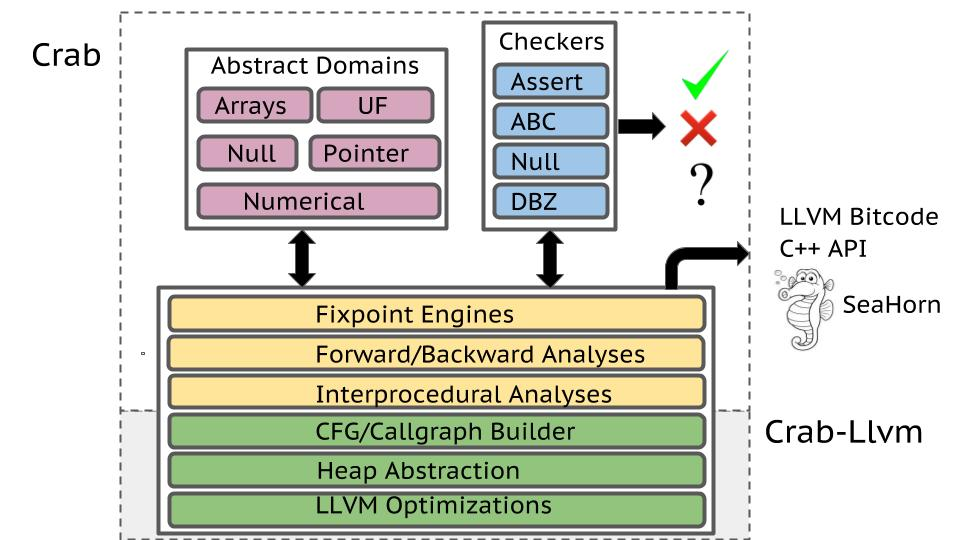
\includegraphics[width=\linewidth]{crabArchitecture}}
\caption{Архитектура Crab-LLVM}
\label{image:crabArchitecture}
\end{figure}

Библиотека Crab и система Crab-LLVM предоставляют большое количество удобных
и полензых инструментов для статического анализа языка C, однако обладают 
следующими ограничениями:
\begin{itemize}
\item при трансляции из LLVM-IR в Crab-CFG игнорируются все операции над 
числами с плавающей точкой;
\item численные абстрактные домены Crab работают над бесконечной числовой 
осью $[-\infty, \infty]$~(а в LLVM целые числа это двоичные числа с 
ограниченной разрядностью);
\item Crab обладает ограниченными возможностями анализа указателей: он может
анализировать содержимое указателей только в том случае, когда ему удается 
статически доказать, что указатель указывает на область памяти, которая ведет 
себя как массив. Для всех остальных указателей он предоставляет только простой
анализ на валидность~(является ли указатель валидным, или указывает на ноль).
\end{itemize}

%%%%%%%%%%%%%%%%%%%%%%%%%%%%%%%%%%%%%%%%%%%%%%%%%%%%%%%%%%%%%%%%%%%%%%%%%%%%%%%
\subsection{Библиотека APRON}
%%%%%%%%%%%%%%%%%%%%%%%%%%%%%%%%%%%%%%%%%%%%%%%%%%%%%%%%%%%%%%%%%%%%%%%%%%%%%%%
APRON~\cite{apron} --- библиотека, которая предоставляет API для работы 
численными абстрактными доменами. Она содержит реализации нескольких
абстрактных доменов для целых чисел и чисел с плавающей точкой. Библиотека 
позиционируется как основа для разработки более продвинутого и глубокого 
анализа. Главным недостатком данной библиотеки является то, что она предоставляет абстрактные домены только для численных значений, нет никаких 
инструментов для работы с массивами, указателями и т.~д.

%%%%%%%%%%%%%%%%%%%%%%%%%%%%%%%%%%%%%%%%%%%%%%%%%%%%%%%%%%%%%%%%%%%%%%%%%%%%%%%
\subsection{Библиотека IKOS}
%%%%%%%%%%%%%%%%%%%%%%%%%%%%%%%%%%%%%%%%%%%%%%%%%%%%%%%%%%%%%%%%%%%%%%%%%%%%%%%
IKOS~\cite{ikos} --- библиотека статического анализа оснванная на теории 
абстрактной интерпретации. Она предназначена для упрощения процесса разработки 
анализаторов. Библиотека предоставляет реализации большого количества 
алгоритмов и структур данных, необходимых при абстрактной интерпретации: 
абстрактные домены, алгоритмы над CFG и т.д. Библиотека IKOS не привязана к
конкретному языку, на ее основе можно построить анализатор для любого языка.
У проекта IKOS есть статический анализатор для языков C/C++, разработанный
в качестве демонстрации применимости предоставляемых инструментов для анализа
реальных программ.

Библиотека предоставляет реализации большого количества абстрактных доменов, в
том числе: численные домены~(интервальный, октагональный и т.д.), домен 
указателей и др. Однако, предоставляемый домен указателей сильно ограничен
по возможностям:
\begin{itemize}
\item он может моделировать только указатели, указывающие на целые числа или
числа с плавающей точкой;
\item не поддерживаются указатели с несколькими уровнями вложенности~(указатели
на указатели).
\end{itemize}

IKOS также предоставляет инструменты для поиска ошибок по результатам 
интерпретации: обнаружение выхода за границы массива, деление на ноль,
разыменование нулевого указателя и т.~д.

Проанализировав вышеописанные библиотеки абстрактной интерпретации для LLVM,
можно выделить следующие их недостатки:
\begin{itemize}
\item наибольшый акцент во всех библиотеках делается на числовые домены. Все 
библиотеки содержат реализации большого количества числовых доменов, как самых
простых и быстрых, так и наиболее точных и ресурсоемких. Однако, все 
библиотеки позволяют работать только с целыми числами на бесконечной числовой
оси. Ни одна из рассмотренных библиотек не позволяет работать с числами с 
фиксированной разрядностью;
\item рассмотренные библиотеки или вообще не поддерживают или очень ограниченно
поддерживают работу с указателями;
\item массивы и структуры поддерживаютя очень ограниченно;
\item ни одна из рассмотренных библиотек не позволяет работать с указателями на функции.
\end{itemize}

Поэтому, было решено разработать свою библиотеку для абстрактной интерпретации
LLVM IR, которая бы удовлетворяла поставленным требованиям.

%%%%%%%%%%%%%%%%%%%%%%%%%%%%%%%%%%%%%%%%%%%%%%%%%%%%%%%%%%%%%%%%%%%%%%%%%%%%%%%
\section{Абстрактные домены для LLVM IR}
%%%%%%%%%%%%%%%%%%%%%%%%%%%%%%%%%%%%%%%%%%%%%%%%%%%%%%%%%%%%%%%%%%%%%%%%%%%%%%%
Одним из главных этапов разработки технологии объединения АИ и BMC является
выбор абстрактных доменов для моделирования переменных LLVM и PS. Необходимо,
чтобы выбранные домены были нересурсоемкими, но обладали приемлемой точностью.
В данном разделе описываются абстрактные домены, выбранные для разработки 
технологии.

%%%%%%%%%%%%%%%%%%%%%%%%%%%%%%%%%%%%%%%%%%%%%%%%%%%%%%%%%%%%%%%%%%%%%%%%%%%%%%%
\subsection{Домены для простых типов данных}
%%%%%%%%%%%%%%%%%%%%%%%%%%%%%%%%%%%%%%%%%%%%%%%%%%%%%%%%%%%%%%%%%%%%%%%%%%%%%%%
Одним из наиболее простых и эффективных доменов для представление целых чисел и
чисел с плавающей точкой является интервальный домен. В этом домене каждая 
переменная $x$ представляется как интервал $[a, b]$ всех значений, которые она 
может принимать. При этом минимальное значение домена $\bot$ соответствует 
пустому интервалу $[]$, максимальное значение $\top = [-\infty, \infty]$. 
Операции объединения и пересечения для интервального домена:
\begin{itemize}
\item $[a, b] \wedge [c, d] = [min(a, c), max(b, d)]$;
\item $[a, b] \vee [c, d] = [max(a, c), min(b, d)]$.
\end{itemize}

Арифметические операции над интервальным доменом достаточно просты:
\begin{itemize}
\item $[a, b] + [c, d] = [a + c, b + d]$;
\item $[a, b] - [c, d] = [a - d, b - c]$;
\item $[a, b] * [c, d] = [min(a * c, b * c, a * d, b * d), max(a * c, b * c,
a * d, b * d)]$;
\item $[a, b] / [c, d] = [min(a / c, b / c, a / d, b / d), max(a / c, b / c,
a / d, b / d)]$;
\end{itemize}

Однако, при использовании интервального домена для целочисленных переменных 
LLVM возникают некоторые особенности. Как упоминалось ранее, целые числа в 
LLVM обладают фиксированной разрядностью, а арифметические и логические 
операции можно выполнять только для чисел с одинаковой разрядностью. Поэтому, 
границы интервала $a$ и $b$ тоже должны быть целочисленными переменными с 
фиксированной разрядностью. Тогда, интервальный домен будет покрывать все 
числа в интервале $[0, 2^i - 1]$~(если считать, что числа беззнаковые), где
$i$ --- разрядность переменной. Более подробно рассмотреть использование
интервального домена для целых чисел в LLVM можно на примере функции из 
листинга~\ref{lst:funcC}. Представление данной функции в LLVM IR приведено в
листинге~\ref{lst:funcLLVM}.

\begin{lstlisting}[style=c, caption={Пример функции на языке С}, 
label=lst:funcC]
int foo(int x) {
    int y;
    if (x > 10) {
        y = x; // y1
    } else {
        y = x - 1; // y2
    }
    return y; // y3 = join(y1, y2)
}
\end{lstlisting}

\begin{lstlisting}[style=llvm, caption={Представление функции из 
    листинга~\ref{lst:funcC} в LLVM IR}, label=lst:funcLLVM]
define i32 @foo(i32 %x) #0 {
entry:
  %cmp = icmp sgt i32 %x, 10
  br i1 %cmp, label %if.then, label %if.else

if.then:
  br label %if.end

if.else:
  %sub = add nsw i32 %x, 4294967295
  br label %if.end

if.end:
  %y.0 = phi i32 [ %x, %if.then ], [ %sub, %if.else ]
  ret i32 %y.0
}
\end{lstlisting}

Предположим, что $x = [0, \top]$, тогда $\%sub = [4294967295, \top]$, $\%y.0 = 
x \wedge \%sub = [0, \top] \wedge [4294967295, \top]$. Из-за того, что в LLVM 
целочисленные переменные не имеют знака, непонятно как интерпретировать данную
операцию объединения:
\begin{itemize}
\item если считать переменные беззнаковыми, то $\%y.0 = [0, \top]$;
\item если считать переменные знаковыми, то $\%y.0 = [4294967295, \top]$.
\end{itemize}

Для того, чтобы решить данную неоднозначность, каждую переменную необходимо
аппроксимировать двумя разными интервалами: один знаковый, другой беззнаковый.
Все операции, у которых не определен знак выполняются два раза: отдельно для
знаковых интервалов, отдельно для беззнаковых. Если у операции определен знак,
то операция выполняется только для соответствующих интервалов~(например, 
операция \texttt{udiv} использует только беззнаковые интервалы, 
\texttt{sdiv} --- только знаковые).

%%%%%%%%%%%%%%%%%%%%%%%%%%%%%%%%%%%%%%%%%%%%%%%%%%%%%%%%%%%%%%%%%%%%%%%%%%%%%%%
\subsection{Агрегатный домен}
%%%%%%%%%%%%%%%%%%%%%%%%%%%%%%%%%%%%%%%%%%%%%%%%%%%%%%%%%%%%%%%%%%%%%%%%%%%%%%%
Массивы и структуры в LLVM представлены схожим образом: это некоторые объекты 
в памяти, доступ к элементам которых можно получить по целочисленному индексу.
Главным отличием этих типов является то, что в массиве все элемены имеют 
одинаковый тип, а в структурах --- разный. Поэтому, при работе со структурами
на индексы, по которым обращаются к полям структуры накладывается ограничение:
они должны быть константами~(чтобы еще на этапе компиляции точно знать какой 
тип будет у всех переменных).

Из-за этих схожестей, можно использовать один домен для аппроксимации и 
структур, и массивов~(при этом, домен сохраняет информацию о том, какой именно
агрегатный тип он аппроксимирует). Агрегатный домен можно реализовывать на 
разных уровнях точночти: от уровня бит и байт до уровня конкретных элементов. 
Соответственно, чем ниже уровень моделирования, чем выше точность и сложность 
домена. Так как в данной работе делается упор на производительность, было 
решено реализовывать агрегатный домен на уровне элементов: каждой переменной 
ставится в соответствие домен, который хранит количество элементов в домене и 
массив всех элементов~(количество элементов представляется в виде интервала, 
массив создается размером с верхнюю грань интервала). Элементы в массиве при 
этом представляются в виде абстрактных доменов соответствующих типов. 
Агрегатный домен поддерживает следующие операции:
\begin{itemize}
\item операция объединения~(рисунок~\ref{image:arrayJoin}).
\begin{figure}[h!]
\textbf{Вход:} $aggregate_1, aggregate_2$ --- объединяемые указатели

\textbf{Выход:} $result$ --- результат объединения двух доменов

\begin{algorithmic}[1]
\State $length \gets aggregate_1.length \wedge aggregate_2.length$
\State $elements \gets array(length.max, \bot)$
\For{$i \in [0, length.max]$}
    \State $elements \gets aggregate_1.elements[i] \wedge
    aggregate_2.elements[i]$
\EndFor
\State $result \gets Aggregate(length, elements)$
\end{algorithmic}
\caption{Алгоритм объединения агрегатных доменов}
\label{image:arrayJoin}
\end{figure}

\item получение указателя на элемент по целочисленным смещениям~(операция 
\texttt{gep}). Операция возвращает указатель на все элементы массива, которые
входят в интервал смещения~(рисунок~\ref{image:arrayGep}).
\begin{figure}[h!]
\textbf{Вход:} $aggregate$ --- агрегатный домен\\
\textbf{Вход:} $shifts$ --- смещения

\textbf{Выход:} $result$ --- указатель на элементы агрегатного домена

\begin{algorithmic}[1]
\State $curShift \cup subShifts \gets shifts$
\State $result \gets \bot$
\If{$subShifts == \emptyset$}
    \State $loc \gets Location({curShift}, this)$
    \State $reslut \gets Pointer({loc})$
\Else
    \For{$i \in [curShift.min, curShift.max]$}
        \State $result \gets result \wedge 
        aggregate.elements[i].gep(subShifts)$
    \EndFor
\EndIf
\end{algorithmic}
\caption{Алгоритм получение указателя на элемент агрегатного домена}
\label{image:arrayGep}
\end{figure}

\item получение элемента по целочисленному смещению~(операции 
\texttt{extractValue}, \texttt{extractElement})~(рисунок~
\ref{image:arrayLoad}).
\begin{figure}[h!]
\textbf{Вход:} $aggregate$ --- агрегатный домен\\
\textbf{Вход:} $shift$ --- смещение

\textbf{Выход:} $result$ --- результат чтения из агрегатного домена

\begin{algorithmic}[1]
\State $result \gets \bot$
\For{$i in [0, aggregate.length.max]$}
    \State $result \gets result \wedge aggregate.elements[i]$
\EndFor
\end{algorithmic}
\caption{Алгоритм чтения значения из агрегатного домена}
\label{image:arrayLoad}
\end{figure}

\item запись значения в элемент по целочисленному смещению~(операции
\texttt{insertValue}, \texttt{insertElement})~(рисунок~\ref{image:arrayStore}).
\begin{figure}[h!]
\textbf{Вход:} $aggregate$ --- агрегатный домен\\
\textbf{Вход:} $shift$ --- смещение\\
\textbf{Вход:} $value$ --- записываемое значение

\begin{algorithmic}[1]
\For{$i in [0, aggregate.length.max]$}
    \State $aggregate.elements[i] \gets aggregate.elements[i] \wedge shift$
\EndFor
\end{algorithmic}
\caption{Алгоритм записи значения в агрегатный домен}
\label{image:arrayStore}
\end{figure}
\end{itemize}

Примеры операций над агрегатным доменом приведены на 
рисунке~\ref{image:aggregateDomain}.
\begin{figure}[h!]
\center{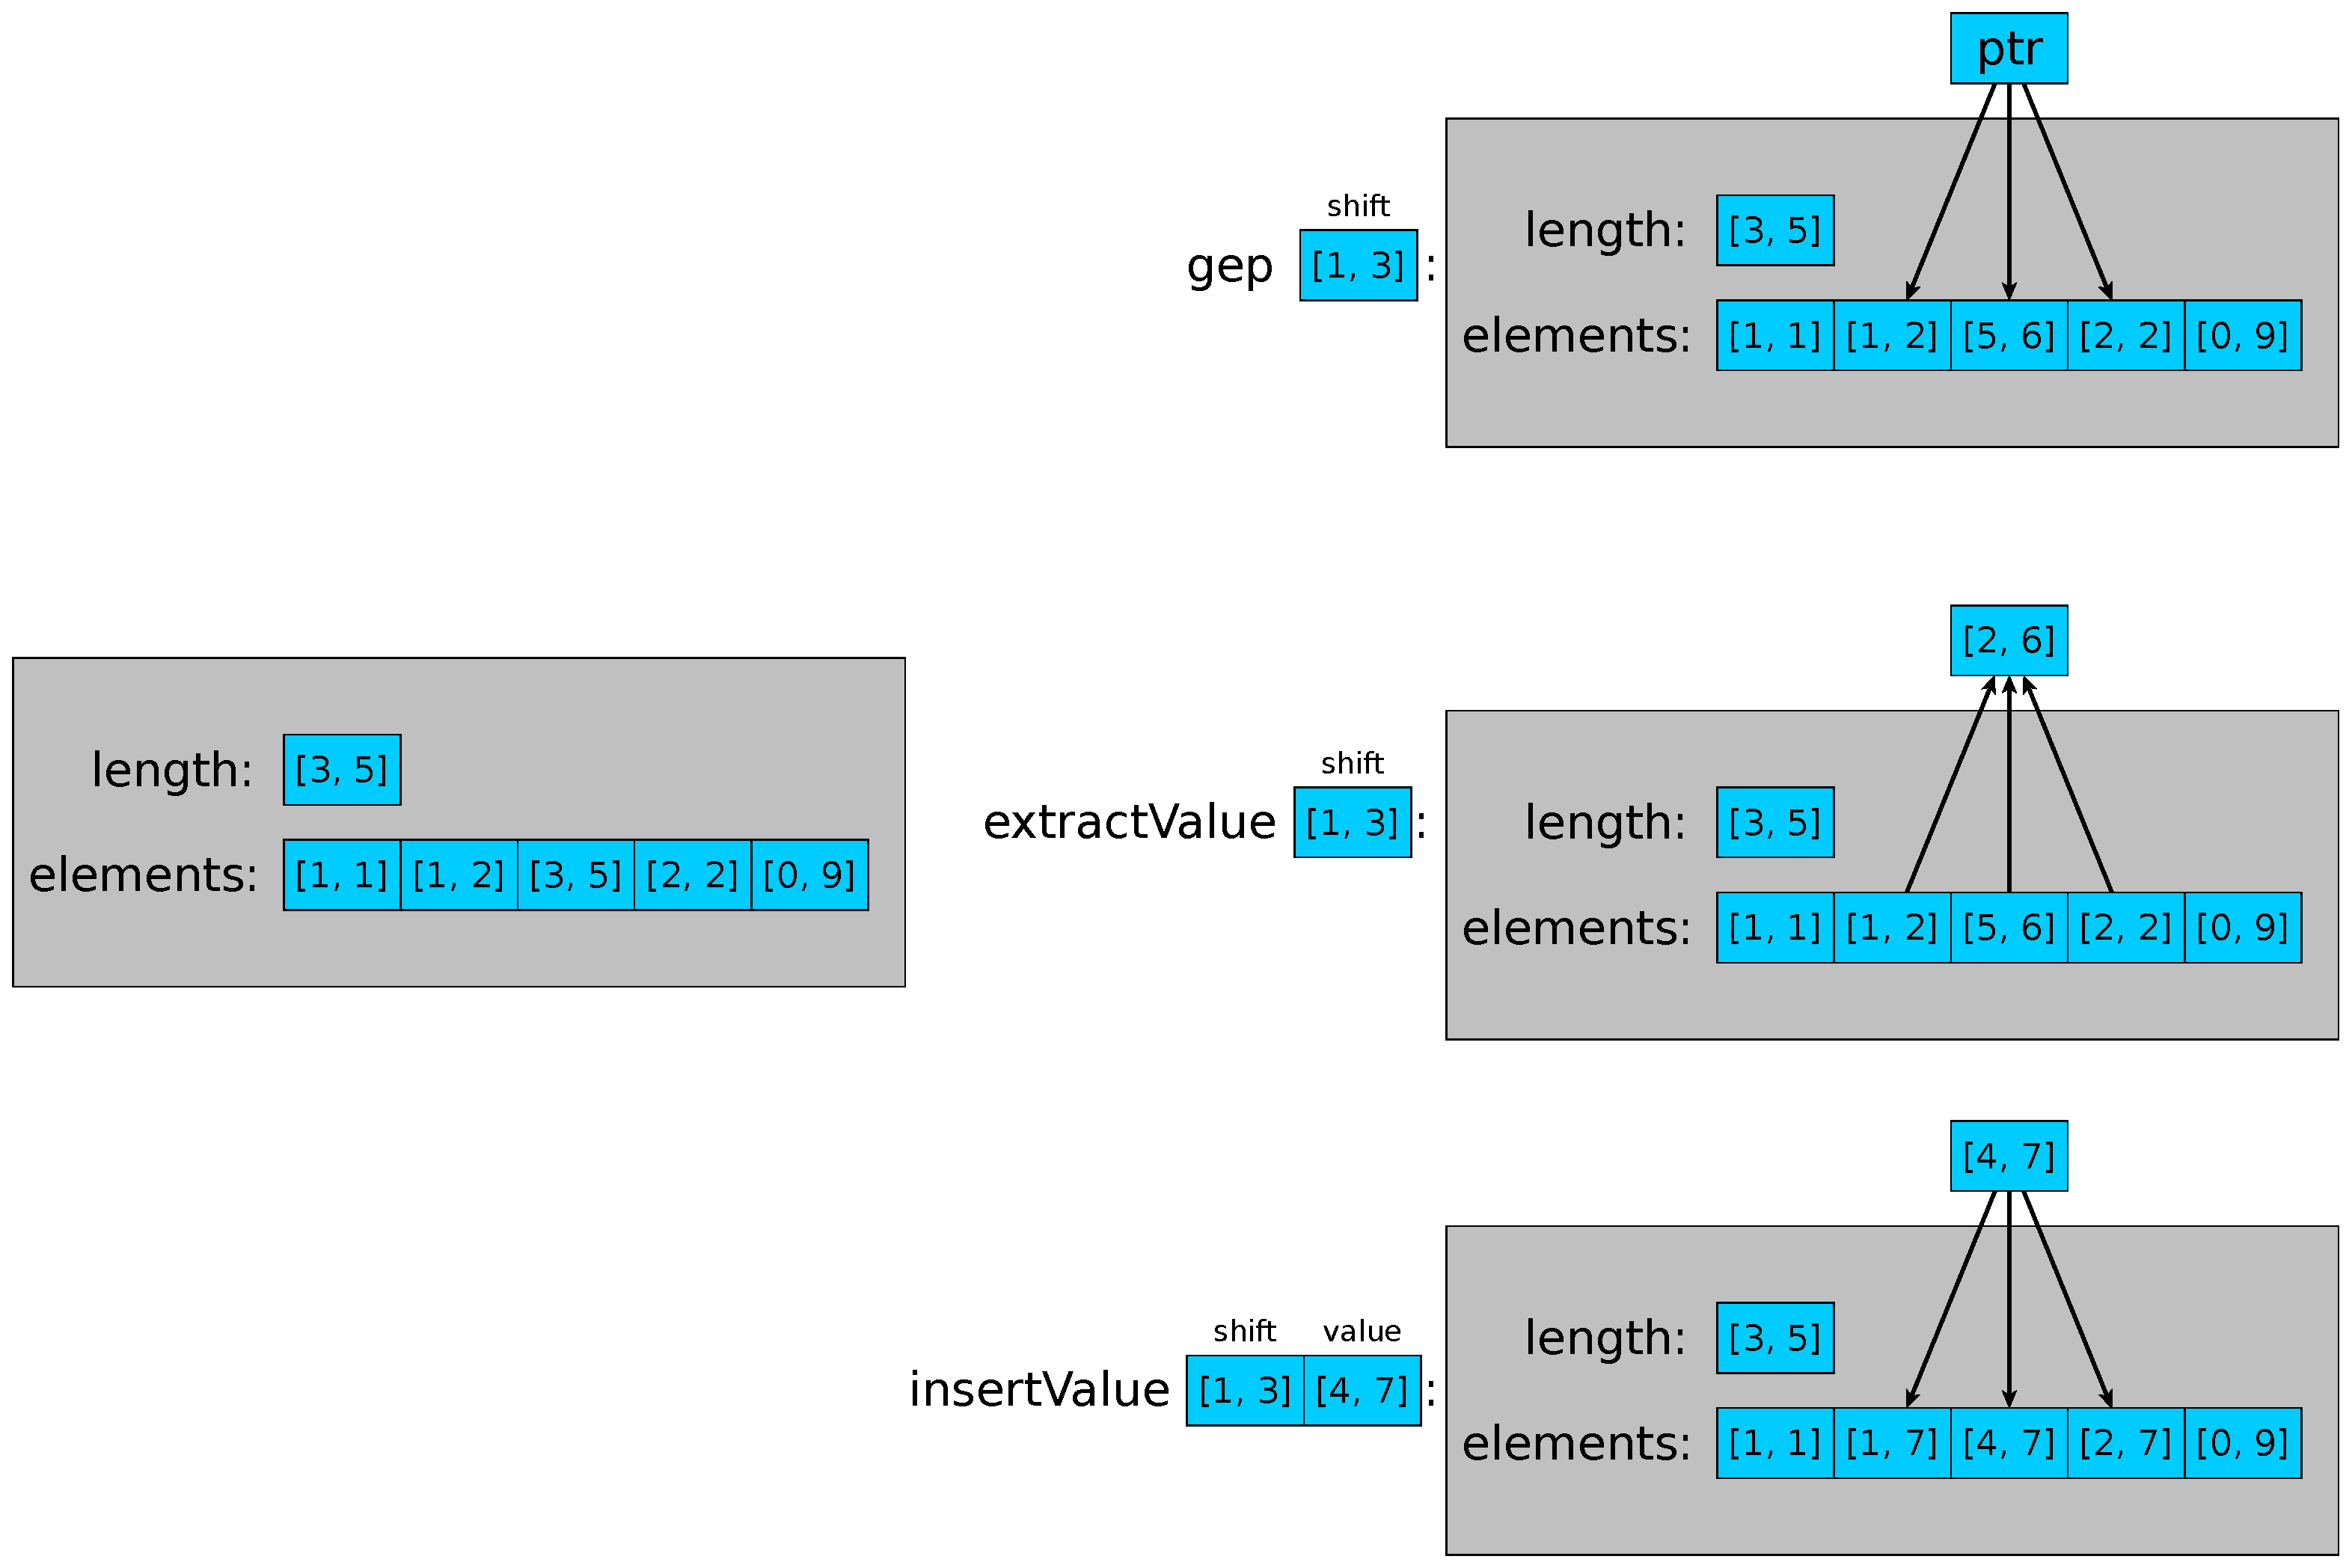
\includegraphics[width=\linewidth]{aggregateDomain}}
\caption{Примеры операций над агрегатным доменом}
\label{image:aggregateDomain}
\end{figure}

%%%%%%%%%%%%%%%%%%%%%%%%%%%%%%%%%%%%%%%%%%%%%%%%%%%%%%%%%%%%%%%%%%%%%%%%%%%%%%%
\subsection{Домен указателей}
%%%%%%%%%%%%%%%%%%%%%%%%%%%%%%%%%%%%%%%%%%%%%%%%%%%%%%%%%%%%%%%%%%%%%%%%%%%%%%%
Каждому указателю в LLVM ставится в соответствие домен, который хранит 
множество локаций. Каждая локация это:
\begin{itemize}
\item объект, на который потенциально может указывать указатель;
\item множество целочисленных смещений относительно начала этого объекта~(в 
виде интервала).
\end{itemize}

Если указатель указывает на массив, то множество смещений можно уменьшить до 
единственного интервала объединив между собой все смещения. Если же указатель
указывает на структуру, необходимо хранить все смещения по отдельности, так
как иначе после объединения этих смещений может получиться указатель, который
ссылается на несколько полей структуры, которые имеют разный тип.

При этом, все объекты на которые указывает домен должны иметь агрегатный тип.
Если указатель в исходной программе указывает на объект простого типа~(например
указатель типа \texttt{int*}), то необходимо преобразовать этот объект в 
агрегатный домен с размером $[1, 1]$ и элементом необходимого типа~(то есть
в массив \texttt{int[1]} для примера). Также, для нулевых указателей
необходимо создать специальный объект \texttt{nullptr\_location}, который 
соответствует 0. Если указатель потенциально указывает на 0, то
\texttt{nullptr\_location} добавляется в множество объектов, на которые он 
может указывать. Пример представления указателей в виде абстрактных доменов
приведен на рисунке~\ref{image:memory}.
\begin{figure}[h!]
\center{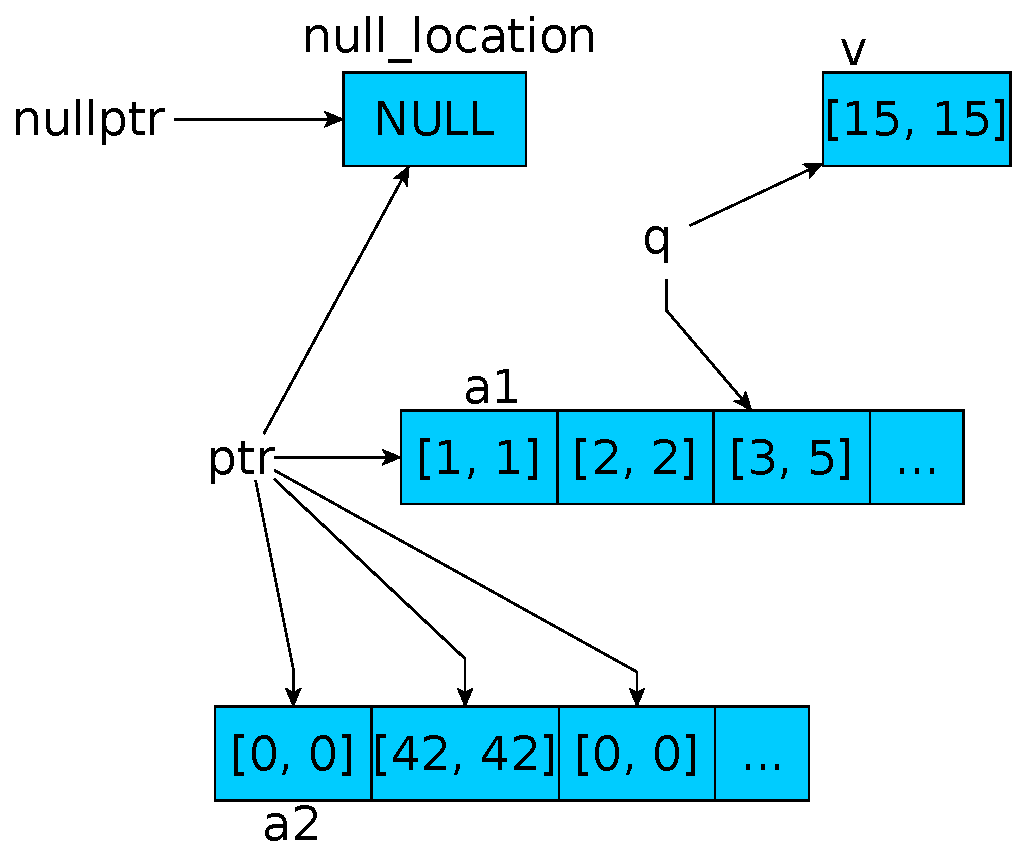
\includegraphics[width=0.7\linewidth]{memory}}
\begin{lstlisting}[style=nostyle]
nullptr = {
    {{[0, 0]}, null_location}
}
q = {
    {{[2, 2]}, a1}
    {{[0, 0]}, v}
}
ptr = {
    {{[0, 0]}, a1}
    {{[0, 2]}, a2}
    {{[0, 0]}, null_location}
}
\end{lstlisting}
\caption{Примеры доменов указателей}
\label{image:memory}
\end{figure}

Домен указателей поддерживает следующие операции:
\begin{itemize}
\item операция объединения. Алгоритм, по которому происходит объединение
двух указателей приведен на рисунке~\ref{image:ptrJoin}. В результате 
объединения двух указателей получается новый указатель, который содержит в 
себе все объекты, на которые указывает хотя бы один из указателей. В строчках 
6 -- 12 обрабатывается ситуация, когда оба указателя указывают на один и тот 
же объект. Если этот объект -- структура, то смещения обоих указателей 
объединяются в одно множество, иначе все эти смещения объединяются в один 
интервал.
\begin{figure}[h!]
\textbf{Вход:} $ptr_1, ptr_2$ --- объединяемые указатели

\textbf{Выход:} $result = ptr_1 \wedge ptr_2$

\begin{algorithmic}[1]
\State $locations \gets \emptyset$
\For{$loc \in ptr_1.locations$}
    \State $loc2 = find(ptr_2.locations, loc)$
    \If{$loc2 \ne null$}
        \State $object \gets loc.object$
        \If{$object.type == Record$}
            \State $shifts \gets loc.shifts \cup loc2.shifts$
            \State $locations \gets locations \cup Location(object, shifts)$
        \Else
            \State $shift \gets loc.shifts[0] \wedge loc2.shifts[0]$
            \State $locations \gets locations \cup Location(object, \{shift\})$
        \EndIf
    \Else
        \State $locations \gets locations \cup loc$
    \EndIf
\EndFor
\State $result \gets Pointer(locations)$
\end{algorithmic}
\caption{Алгоритм объединения домена указателей}
\label{image:ptrJoin}
\end{figure}

\item операция чтения значения из указателя по смещению~(операция 
\texttt{load})~(рисунок~\ref{image:ptrJoin}).
\begin{figure}[h!]
\textbf{Вход:} $ptr$ --- указатель\\
\textbf{Вход:} $shift$ --- смещение

\textbf{Выход:} $result$ --- результат чтения из указателя по указанному 
смещению 

\begin{algorithmic}[1]
\State $result \gets \bot$
\For{$loc \in ptr.locations$}
    \For{$curShift \in loc.shifts$}
        \State $totalShift \gets curShift + shift$
        \State $result \gets result \wedge loc.extractValue(totalShift)$
    \EndFor
\EndFor
\end{algorithmic}
\caption{Алгоритм чтения значения из указателея}
\label{image:ptrJoin}
\end{figure}

\item операция записи значения в указатель по смещению~(операция 
\texttt{store})~(рисунок~\ref{image:ptrStore}).
\begin{figure}[h!]
\textbf{Вход:} $ptr$ --- указатель\\
\textbf{Вход:} $shift$ --- смещение\\
\textbf{Вход:} $value$ --- записываемое значение

\begin{algorithmic}[1]
\For{$loc \in ptr.locations$}
    \For{$curShift \in loc.shifts$}
        \State $totalShift \gets curShift + shift$
        \State $loc.insertValue(totalShift, value)$
    \EndFor
\EndFor
\end{algorithmic}
\caption{Алгоритм чтения значения из указателея}
\label{image:ptrStore}
\end{figure}

\item операция получения указателя на хранимые объекты по смещениям~(операция 
\texttt{gep})~(рисунок~\ref{image:ptrGep}).
\begin{figure}[h!]
\textbf{Вход:} $ptr$ --- указатель\\
\textbf{Вход:} $shifts$ --- смещение\\

\textbf{Выход:} $result$ --- указатель на хранимые объекты по смещениям

\begin{algorithmic}[1]
\State $result \gets \bot$
\State $curShift \cup subShifts \gets shifts$
\For{$loc \in ptr.locations$}
    \For{$curShift \in loc.shifts$}
        \State $curShifts \gets \{curShift\} \cup subShifts$
        \State $result \gets result \wedge loc.gep(curShifts)$
    \EndFor
\EndFor
\end{algorithmic}
\caption{Алгоритм получения указателя на хранимые объекты}
\label{image:ptrGep}
\end{figure}

\item операция сравнения указателей на равенство~(рисунок~\ref{image:ptrEq}).
При сравнении двух указателей на равенство можно обработать только некоторые
частные случаи. Результатом сравнения двух указателей будет интервальный домен разрядности 1.
\begin{figure}[h!]
\textbf{Вход:} $ptr_1, ptr_2$ --- указатели

\textbf{Выход:} $result$ --- результат сравнения

\begin{algorithmic}[1]
\State $result \gets \bot$
\If{$ptr_1 == ptr_2$}
    \State $result \gets IntegerInterval(1, 1)$
\ElsIf{$ptr_1.isNull() \&\& ptr_2.isNull()$}
    \State $result \gets IntegerInterval(1, 1)$
\ElsIf{$ptr_1.locations \cap ptr_2.locations == \emptyset$}
    \State $result \gets IntegerInterval(1, 0)$
\Else
    \State $result \gets \top$
\EndIf

\end{algorithmic}
\caption{Алгоритм получения указателя на хранимые объекты}
\label{image:ptrEq}
\end{figure}

\item операция сравнения указателей на неравенство~(выражается через операцию
сравнения на равенство).
\end{itemize}

%%%%%%%%%%%%%%%%%%%%%%%%%%%%%%%%%%%%%%%%%%%%%%%%%%%%%%%%%%%%%%%%%%%%%%%%%%%%%%%
\subsection{Домен функций}
%%%%%%%%%%%%%%%%%%%%%%%%%%%%%%%%%%%%%%%%%%%%%%%%%%%%%%%%%%%%%%%%%%%%%%%%%%%%%%%
В языке C достаточно часто используются указатели на функции и, соответственно,
вызов функции по указателю. Этот механизм дает большие возможности при 
разработке программ: реализация параметризируемых алгоритмов, обратных 
вызовов~(callback), некое подобие виртуальных функций для структур. Однако, 
указатели на функции создают большие проблемы при анализе: невозможно точно 
сказать какая конкретно функиця вызывается в той или иной инструкции.

Домен указателей на функцию хранит:
\begin{itemize}
\item прототип функции, на которую он указывает~(тип возвращаемого значения
и типы аргументов функции);
\item множество функций, на которые он потенциально указывает~(каждая функция
этого множества соответствует прототипу). Если домен имеет значение $\top$, в
данное множество добавляются все функции, объявленные в текущем модуле и 
соответствующие прототипу.
\end{itemize}

Объединение двух доменов функций возвращает новый домен, в котором содержится
объединение множеств функций первого и второго домена.